\documentclass[a4paper]{scrreprt}

% Uncomment to optimize for double-sided printing.
% \KOMAoptions{twoside}

% Set binding correction manually, if known.
% \KOMAoptions{BCOR=2cm}

% Localization options
\usepackage[english]{babel}
\usepackage[T1]{fontenc}
\usepackage[utf8]{inputenc}

% Sub figures
\usepackage{subcaption}

% Quotations
\usepackage{dirtytalk}

% Floats
\usepackage{float}

% Algorithms using algorithmicx package (with its algpseudocode command set)
\usepackage{algorithm}
\usepackage{algpseudocode}

% Enhanced verbatim sections. We're mainly interested in
% \verbatiminput though.
\usepackage{verbatim}

% Automatically remove leading whitespace in lstlisting
\usepackage{lstautogobble}

% CSV to tables
\usepackage{csvsimple}

% PDF-compatible landscape mode.
% Makes PDF viewers show the page rotated by 90°.
\usepackage{pdflscape}

% Advanced tables
\usepackage{array}
\usepackage{tabularx}
\usepackage{longtable}

% Fancy tablerules
\usepackage{booktabs}

% Graphics
\usepackage{graphicx}

% Current time
\usepackage[useregional=numeric]{datetime2}

% Float barriers.
% Automatically add a FloatBarrier to each \section
\usepackage[section]{placeins}

% Custom header and footer
\usepackage{fancyhdr}

\usepackage{geometry}
\usepackage{layout}

% Math tools
\usepackage{mathtools}
% Math symbols
\usepackage{amsmath,amsfonts,amssymb}
\usepackage{amsthm}
% General symbols
\usepackage{stmaryrd}

% Utilities for quotations
\usepackage{csquotes}

% Bibliography
\usepackage[
  style=alphabetic,
  backend=biber, % Default backend, just listed for completness
  sorting=ynt % Sort by year, name, title
]{biblatex}
\addbibresource{references.bib}

\DeclarePairedDelimiter\abs{\lvert}{\rvert}
\DeclarePairedDelimiter\floor{\lfloor}{\rfloor}
\DeclarePairedDelimiter\ceil{\lceil}{\rceil}

% Custom operators
\DeclareMathOperator{\fft}{FFT}
\DeclareMathOperator{\dft}{DFT}
\DeclareMathOperator{\dwt}{DWT}
\DeclareMathOperator{\intdiv}{div}

% Sets!
\newcommand{\setnat}{\mathbb{N}}
\newcommand{\setint}{\mathbb{Z}}

% Various math
\newcommand{\fermatnum}[1]{F_{#1}}

% Bullet point
\newcommand{\tabitem}{~~\llap{\textbullet}~~}

\pagestyle{plain}
% \fancyhf{}
% \lhead{}
% \lfoot{}
% \rfoot{}
% 
% Source code & highlighting
\usepackage{listings}

% SI units
\usepackage{siunitx}

\newcommand{\lecture}{41862 - Seminar Advanced Algorithms}
% Convenience commands
\newcommand{\mailsubject}{\lecture - Report}
\newcommand{\maillink}[1]{\href{mailto:#1?subject=\mailsubject}
                               {#1}}

% Should use this command wherever the print date is mentioned.
\newcommand{\printdate}{\today}

\subject{\lecture}
\title{Schönhage-Strassen algorithm for fast integer multiplication}

\author{Michael Senn \maillink{michael.senn@students.unibe.ch} --- 16-126-880}

\date{\printdate}

% Needs to be the last command in the preamble, for one reason or
% another. 
\usepackage{hyperref}

\begin{document}

\maketitle

\begin{abstract}
		% TODO
		This report serves as an introduction to the fast integer multiplication algorithm described by Schönhage and Strassen.
\end{abstract}

\chapter{Introduction}
\label{chapter:introduction}

This report aims to provide the reader an introduction into the fast integer
multiplication algorithm proposed by Schönhage and Strassen in 1971.
\autocite{schonhageSchnelleMultiplikationGrosser1971}

It will start with a discussion of the problem to be solved and historical
solutions in chapter \ref{chapter:introduction}. Chapter
\ref{chapter:mathematical_background} will introduce the required mathematical
background, with a focus on convolution theory and the Discrete Fourier
Transform.. Chapter \ref{chapter:integer_multiplication_convolution} will show
how to model the problem of integer multiplication as a convolution problem,
along with a basic algorithm to solve it. Chapter
\ref{chapter:schoenhage_strassen} will then introduce the Schönhage-Strassen
algorithm, and explain various of its details. Finally we will conclude in
chapter \ref{chapter:conclusion}.

\section{Problem statement}

The problem the Schönhage-Strassen algorithm intends to solve is to, given two
integers $x, y \in \mathbb{Z}$, calculate their product $z \coloneqq x \cdot
y$.

\section{Historical development}

\subsection{Long multiplication}

One of the most common algorithms for multiplication taught in school is known
as `long multiplication'. Given a representation of the multiplicand and
multiplier in some base --- commonly base 10 --- each digit of the multiplicand
is multiplied by each digit of the multiplier. All intermediary products
encoding for the same digit of the chosen base will then be summed up. Finally
a potential carry propagation takes place, yielding a representation of the
product in the chosen base.

It is trivial to see that this algorithm requires $O(n^2)$ multiplication and
additions.

\subsection{Work leading up to Schönhage-Strassen}

For a while it had been conjectured that an asymptotic complexity $\Omega(n^2)$
was ideal for the problem of integer multiplication. In 1962, Karatsuba found
an algorithm where one multiplication of two $2n$-digit numbers could be
replaced with three multiplications of $n$-digit numbers. This lead to an
asymptotic complexity of $\approx O(n^{1.58})$. In 1963 and 1966, Toom and Cook
generalised Karatsuba's approach to a complexity of $O(n^{1.46})$. In 1971
finally, Schönhage and Strassen proposed an algorithm with complexity $O(n
\log(n) \log(\log(n)))$ which we will discuss
here.


\chapter{Mathematical background}
\label{chapter:mathematical_background}

This chapter will provide a brief introduction into the discrete Fourier
transform and discrete weighted transform, along with a way to efficiently
calculate either by means of the fast Fourier transform. It will then provide
an introduction into convolution theory, and show how convolutions and the
discrete Fourier transform are linked.

\section{Notation}

The following defines notation used throughout the report.

\section{Discrete Fourier Transform}

The Discrete Fourier Transform (``DFT'') allows performing Fourier analysis of
a discrete $n$-length signal $x = (x_0, x_1, \ldots, x_{n-1})$ over some
algebraic field. Its result is the the $n$-length signal $X$, whose components
are as follows:\autocite{crandallPrimeNumbersComputational2005}

\[
		\dft(x) : X_k = \sum_{j=0}^{n-1} x_j \cdot g^{-jk}
\]

Where $g$ is a primitive $n$-th root of unity of the algebraic field, which is
to say that for some $n \in \setnat$:

\[
		g^n = 1 \land g^m \neq 1\ \forall m < n
\]

The inverse DFT is defined equivalently as the $n$-length signal $x$ whose
components are as follows:

\[
		\dft^{-1}(X) : x_j = \frac{1}{n} \sum_{k=0}^{n-1} X_k \cdot g^{jk}
\]

Such that $\dft^{-1}(\dft(x)) = x$ for all discrete signals $x$.

\subsection{Calculation via fast Fourier Transform}

The naive approach to calculate the DFT would require $O(k^2)$ multiplications
and additions. However it can be shown that the DFT can be efficiently
calculated by means of the Fast Fourier Transform (``FFT'') algorithm, which
has a complexity of $O(n \log(n))$:\autocite{crandallPrimeNumbersComputational2005}

\[
		\dft(x) = \fft(x)
\]

\section{Discrete Weighted Transform}

We further introduce the forward and inverse Discrete Weighted Transform
(``DWT'') of a discrete $n$-length signal $x$ and $n$-length weight vector $a$,
defined to be the $n$-length signal $X$ with components as follows:

\begin{align*}
		\dwt(x, a) & : X_k = \sum_{j=0}^{n-1} (a_j x_j) \cdot g^{-jk} \\
		\dwt^{-1}(X, a) & : x_j = \frac{1}{n a_j} \sum_{k=0}^{n-1} X_k \cdot g^{jk}
\end{align*}

Again with $g$ a primitive $n$-th root of unity of the field.

Clearly from the definition it follows that $\dwt(x, a) = \dft(a \cdot x)$,
where $\cdot$ denotes component-wise multiplication in the algebraic field.
This also implies that $\dwt(x, 1) = \dft(x)$.

\section{Convolution theory}

We now introduce the concept of a convolution --- an operation $*$ on two
functions $f$ and $g$ producing a third function $f * g$:

\[
		(f * g)(t) = \int_{-\infty}^{\infty} f(\tau) \cdot g(t - \tau) d\tau
\]

As we work with discrete rather than continuous signals however, we will
introduce a set of different discrete convolution operations. For the following
paragraphs, assume $x$ and $y$ to be two $n$-length discrete signals.

\subsection{Cyclic convolution}

The cyclic convolution $z = x \times y$ is defined as the $n$-length signal
with components as follows. It is visualized in figure
\ref{fig:cyclic_convolution}:

\[
		z_k \coloneqq \sum_{i + j \equiv k \pmod{n}} x_i \cdot y_i
\]

\subsection{Weighted cyclic convolution}

The weighted cyclic convolution $z = x \times_a y$, with an $n$-length weight
vector $a$, is defined as the $n$-length signal with components as follows.

\[
		z_k = \frac{1}{a_k} \sum_{i + j \equiv k \pmod{n}} (x_i a_i) \cdot (y_j a_j)
\]

\subsection{Acyclic convolution}

The acyclic convolution $u = x \times_A y$ is defined as the $2n$-length signal
with components as follows. It is visualized in figure
\ref{fig:acyclic_convolution}:

\begin{align*}
		u_k & \coloneqq \sum_{i + j = k} x_i \cdot y_i \\
		u_{2n - 1} & \coloneqq 0
\end{align*}

\subsection{Halfcyclic convolution}

The halfcylic convolution $w = x \times_H y$ is defined as the $n$-length
signal consisting of the first $n$ components of the acylic convolution $x
\times_A y$. It is visualized in figure \ref{fig:halfcyclic_convolution}:

\[
		w_k \coloneqq (x \times_A y)(k)
\]

\subsection{Negayclic convolution}

The negacylic convolution $v = x \times_\_ y$ is defined as the $n$-length signal
with components as follows. It is visualized in figure
\ref{fig:negacyclic_convolution}:

\[
		v_k \coloneqq \sum_{i + j = n} x_i \cdot y_i - \sum_{i + j = n + k} x_i \cdot y_i
\]

It can be seen that the negacylic convolution splits the summands of each
signal component of the cyclic convolution into those where the modular
addition operation of the indices `wrapped around', and those where it did not.
Those where it wrapped around are then subtracted from the sum of those where
it did not.

\begin{figure}
		\centering
		\begin{subfigure}{.33\textwidth}
				\centering
				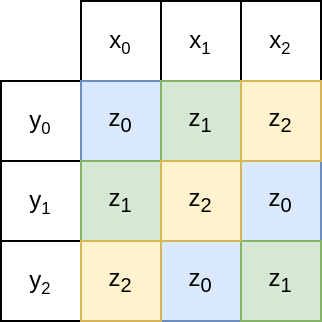
\includegraphics[width=0.9\textwidth]{../resources/cyclic_convolution.drawio.png}
				\caption{Cyclic convolution}
				\label{fig:cyclic_convolution}
		\end{subfigure}%
		\begin{subfigure}{.33\textwidth}
				\centering
				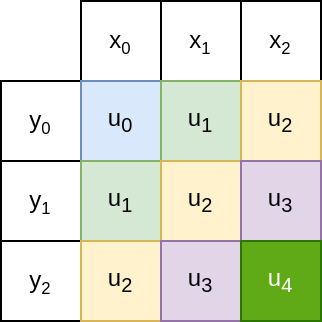
\includegraphics[width=0.9\textwidth]{../resources/acyclic_convolution.drawio.png}
				\caption{Acyclic convolution}
				\label{fig:acyclic_convolution}
		\end{subfigure}%
		\begin{subfigure}{.33\textwidth}
				\centering
				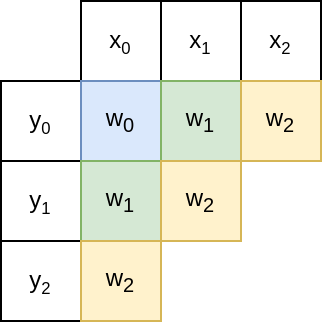
\includegraphics[width=0.9\textwidth]{../resources/halfcyclic_convolution.drawio.png}
				\caption{Halfcyclic convolution}
				\label{fig:halfcyclic_convolution}
		\end{subfigure}
		\begin{subfigure}{.66\textwidth}
				\centering
				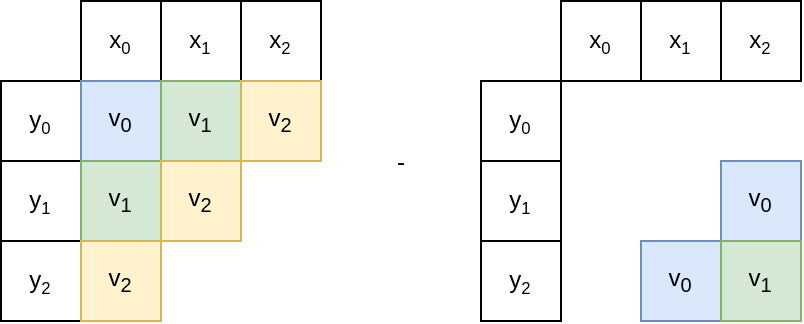
\includegraphics[width=0.9\textwidth]{../resources/negacyclic_convolution.drawio.png}
				\caption{Negacyclic convolution}
				\label{fig:negacyclic_convolution}
		\end{subfigure}
		\caption{
				Different types of discrete convolutions. The input signals $x
				= (x_0, x_1, x_2)$ and $y = (y_0, y_1, y_2)$ are shown along
				the axes. The `cross product' of the input signals represents
				components of the convolution's output, with  labels and
				colours indicating towards which component of the output the
				respective product contributes.  Unless specified otherwise,
				each output signal component is the sum of all products with
				the corresponding label and colour.
}
\end{figure}

\subsection{Relations between convolutions}
\label{sec:relations_between_convolutions}

Various relations between the different types of convolutions exist. One we
will use is the following. Let $L(x)$ be the left half of an even-length
signal. That is if $x = (x_1, x_2, \ldots, x_{2n})$, then $L(x) = (x_1, x_2,
\ldots, x_n)$. Consider now two length-$2n$ signals $x, y$, with the upper half
of either signal being $0$. That is $x_i = y_i = 0, n + 1 \leq i \leq 2n$. Then
it holds that: \autocite{crandallPrimeNumbersComputational2005}

\[
		L(x) \times_A L(y) = x \times y = x \times_\_ y = x \times_H y
\]

These equalities all follow directly from the definition of the convolutions,
using the fact that the upper halves of the input signals are equal to zero.

% Equality of the cyclic and half-cyclic convolution follows directly from their
% definition. They only differ in whether products containing the upper halves of
% the input signals are added to the output signal or not. As the upper halves of
% the input signals are zero however, the two convolutions are equal.
% 
% Equality of the cyclic and negacyclic follows equivalently in that they only
% differ in whether the products containing the upper halves are added or
% subtracted.
% 
% Equality of the half-cyclic of the full and acylic of the lower halves of the
% input signals then follows as seen earlier, in that the half-cyclic is equal to
% the left half of the acyclic of the full.

\subsection{Convolution theorem}
\label{sec:convolution_theorem}

It can further be shown that the cyclic convolution and weighted cyclic
convolution can be calculated by means of the DFT and DWT:
\autocite{crandallPrimeNumbersComputational2005}

\begin{align*}
		x \times y & = \dft^{-1}(\dft(x) \cdot \dft(y)) \\
		x \times_a y & = \dwt^{-1}(\dwt(x, a) \cdot \dwt(y, a), a)
\end{align*}

Where $\cdot$ denotes component-wise multiplication. This allows calculation of
convolutions with complexity $O(n \log(n))$.

By choosing an appropriate weight vector $a$, this also allows the calculation
of other convolutions. Consider choosing the weight vector $a = (a_j) = A^j$
for a scalar $A$. As described by Crandall and Fagin
\autocite{crandallDiscreteWeightedTransforms1994}, the weighted cyclic
convolution of two length-$n$ signals will then take on the following form:

\[
		x \times_a y = (x \times_H y)  + A^n (x \times y - x \times_H y)
\]

Assume then that $A$ is a primitive $2n$-th root of unity. That is $a^{2n} = 1
\Rightarrow a^n = -1$. Then clearly the result of the weighted cyclic
convolution will be the negacyclic convolution:

\[
		x \times_a y = (x \times_H y) - (x \times y - x \times_H y) = 2 \cdot (x \times_H y) - (x \times y) = x \times_\_ y
\]


\chapter{Modelling integer multiplication as a convolution problem}
\label{chapter:integer_multiplication_convolution}

We now aim to show how the problem of integer multiplication can be phrased as
a convolution problem, and then present a basic algorithm to perform integer
multiplications using the FFT.

Consider $x, y$ two $n$-digit numbers in some base $B$, where $x_0, y_0$ is the
least significant digit.

\section{Integer multiplication as a convolution operation}

Let $\otimes$ be an integer multiplication with delayed carry operation. That
is $u = x \otimes y$ is defined as follows:

\begin{align*}
		u_i & = \sum_{j + k = i} x_j y_k
\end{align*}

Observe how by this definition the operation $u = x \otimes y$ is exactly the
acyclic convolution $u = x \times_A y$. This is further illustrated in figure
\ref{fig:multiplication_convolution}.

\begin{figure}
		\centering
		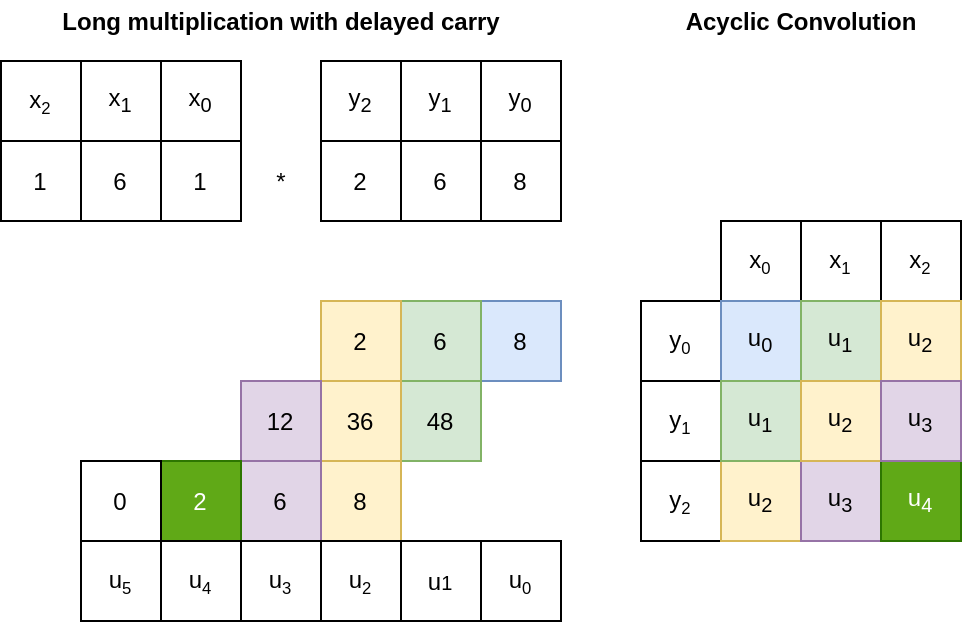
\includegraphics[width=0.6\textwidth]{../resources/multiplication_convolution.drawio.png}
		\caption{Integer multiplication with delayed carry operation is equivalent to acyclic convolution}
		\label{fig:multiplication_convolution}
\end{figure}

\subsection{Applying the delayed carry operation}

Given $u = x \otimes y$, one can calculate the result of a regular
multiplication $v = x \cdot y$ by applying the carry operation. Let
$\intdiv$ denote integer division:

\begin{align*}
		\overline{v}_i & = u_i + (\overline{v}_{i-1} \intdiv B) \\
		v_i & = \overline{v}_i \bmod B
\end{align*}

\section{Integer multiplication with the FFT}

This now allows specification of a basic algorithm for fast integer
multiplication using the FFT, as done by e.g. Crandall and Pomerance, shown in
algorithm \ref{alg:fft_int_mult}.

The algorithm starts by zero-padding the two input signals to length $2n$, and
then calculates $\dft^{-1}(\dft(x_{\text{padded}}) \cdot
\dft(y_{\text{padded}}))$.  Recall that as per sections
\ref{sec:relations_between_convolutions} and \ref{sec:convolution_theorem} this
will thus --- after the rounding required as this generic FFT operates over the
field of complex numbers --- yield the acyclic convolution $x \times_A y$.

The algorithm will then perform the carry operation outlined above, returning
the result $z = x \cdot y$.

\begin{algorithm}
		\caption{Fast integer multiplication with FFT}
		\begin{algorithmic}[1]
				\Function{FFTMult}{$x, y$}
				\State $x \gets$ \Call{Pad}{x, 2n} \Comment{Zero-pad to length $2n$ on high-order side}
				\State $y \gets$ \Call{Pad}{y, 2n}
				\\
				\State $X \gets$ \Call{DFT}{x}
				\State $Y \gets$ \Call{DFT}{y}
				\State $Z \gets X \cdot Y$ \Comment{Dyadic product}
				\State $z \gets$ $\Call{DFT}{Z}^{-1}$
				\State $z \gets$ \Call{round}{z}
				\\
				\State $carry \gets 0$
				\For{$i \gets 0$ to $2n$}
				\State $v \gets z_i + carry$
				\State $z_n \gets v \bmod B$
				\State $carry \gets v \intdiv B$
				\EndFor
				\State \textbf{Return} $z_0 || z_1 || \ldots || z_n || carry$
				\\
				\EndFunction
		\end{algorithmic}
		\label{alg:fft_int_mult}
\end{algorithm}


\chapter{Schönhage-Strassen algorithm for integer multiplication}
\label{chapter:schoenhage_strassen}

\section{Motivation}

While the basic algorithm shown before is functional in terms of pure
mathematics, it is not ideal for implementation in software or hardware. Its
reliance on floating-point arithmetic both introduces the potential for
rounding errors, as well as being generally slow.

The algorithm proposed by Schönhage and Strassen will thus work in
$\setint_{2^n + 1}$, that is the ring of integers modulo $2^n + 1$. This has
the advantage of only utilizing integer arithmetic, which is fast and prevents
rounding errors.

\subsection{Non-modular multiplication}

Note that his is not a limitation if one wants to calculate the non-modular
product. As hinted at by Crandall and Pomerance,
\autocite{crandallPrimeNumbersComputational2005} a choice of $n \geq
\ceil{\log_2(x)} + \ceil{\log_2(y)}$ will ensure that $xy < 2^n + 1$, so the
product modulo $2^n + 1$ will be equal to the non-modular product:
\begin{align*}
		xy & < 2^{\ceil{\log_2(xy)}} + 1 \\
		   & \leq 2^{\ceil{\log_2(x)} + \ceil{\log_2(y)}} + 1 \\
		   & \Rightarrow xy < 2^n + 1
\end{align*}

\section{Algorithm}

We will now present the algorithm as described by Crandall and Pomerance
\autocite{crandallPrimeNumbersComputational2005} piece by piece, providing
explanations and references as to what each section does.

Let $0 \leq x, y < 2^n + 1$ be two integers we wish to multiply modulo $2^n +
1$.

\subsection{Splitting inputs into smaller parts}

In a first step shown in algorithm \ref{alg:ssmult_split_inputs}, the inputs
$x$ and $y$ are split into $D$ parts of length $M$ bits each. As such, $X$ and
$Y$ as shown will thus be a base-$2^M$ representation of $x$ and $y$
respectively.

In order for the recursion to make progress, we then pick an auxiliary modulus
$2^{n'} + 1$. This modulus is chosen large enough such that no component of the
subsequent negacyclic convolution will be reduced. Indeed observe that if $Z = X
\times_\_ Y$, then:
\begin{align*}
		Z_i & \leq D \cdot \max(X_i Y_j) && \text{By the definition of the negacyclic convolution} \\
			& \leq D \cdot \max(X_i) \cdot \max(Y_j) \\
			& < D \cdot 2^M \cdot 2^M && \text{As a result of how $x, y$ were split into $X, Y$} \\
			& = D \cdot 2^{2M}
\end{align*}
And so indeed $\log_2(Z_i) < \log_2(D) + \log_2(2^{2M}) = k + 2M$, such that we
can subsequently work modulo $2^{n'} + 1$ without falsifying the result.

Note that $n'$ is chosen as an integer multiple of $D = 2^k$. This ensures
that, when applied recursively, the requirement that $D | n$ in line
\ref{algline:d_divides_n} of algorithm \ref{alg:ssmult_split_inputs} will hold.

\begin{algorithm}
		\caption{Schönhage-Strassen integer multiplication: Split inputs}
		\begin{algorithmic}[1]
				\Function{Schönhage-Strassen-Mult}{$x, y$}
				\State $D \gets 2^k$ such that $D | n$
				\label{algline:d_divides_n}
				\State $M \gets 2^l$ such that $DM = n$
				\State Pick smallest $n' \geq 2M + k$ such that $n' = DM'$
				\State $X \gets $\Call{Split}{x, D}
				\State $Y \gets $\Call{Split}{y, D}
				\algstore{ssmult}
		\end{algorithmic}
		\label{alg:ssmult_split_inputs}
\end{algorithm}

\subsection{Calculate negacylcic convolution}

We now will calculate the negacyclic convolution $Z = X \times_{\_} Y$. Recall
that as per section \ref{sec:convolution_theorem} this can be achieved via the
weighted cyclic convolution, using a weight vector $(a_i) = A^i$ where $A$ is a
$2D$-th root of unity.

Note that we choose the negacyclic rather than the cyclic convolution since, as
seen in section \ref{sec:modular_integer_multiplication_convolution}, this will
allow us to calculate the reduction modulo $2^n + 1$ `for free'.

Observe first that $2^{2M'}$ is a $D$-th root of unity modulo $2^{n'} + 1$:
\begin{align*}
		(2^{2M'})^D - 1 & = 2^{2M'D} - 1\\
						& = 2^{2n'} - 1 \\
						& = (2^{n'} + 1) (2^{n'} - 1) \\
						& \Rightarrow (2^{2M'})^D \equiv 1 \pmod{2^{n'} + 1}
\end{align*}

And so $A \coloneqq 2^{M'}$ is a $2D$-th root of unity modulo $2^{n'} + 1$ as
required. We will thus first weight each component $X_i$ and $Y_i$ with $A^i$,
shown in algorithm \ref{alg:ssmult_weight_inputs}.

Having the root of unit be a power of two allows multiplications and divisions
with it --- as are required for e.g. the DWT and FFT --- to be done very
efficiently as bit shifts.

\begin{algorithm}
		\caption{Schönhage-Strassen integer multiplication: Weight inputs with $2D$-th root of unity}
		\begin{algorithmic}[1]
				\algrestore{ssmult}
				\For{$i \gets 0, D$}
				\State $X_i \gets (2^{iM'} X_i) \bmod (2^{n'} + 1)$
				\State $Y_i \gets (2^{iM'} Y_i) \bmod (2^{n'} + 1)$
				\EndFor
				\algstore{ssmult}
		\end{algorithmic}
		\label{alg:ssmult_weight_inputs}
\end{algorithm}

We will then apply the $\dft$ to each of $X$ and $Y$, and perform the
component-wise multiplication, shown in algorithm \ref{alg:ssmult_dft}. This
component-wise multiplication can be done with any multiplication algorithm. As
such one can e.g.  recursively use the Schönhage-Strassen algorithm as long as
inputs are large, and then default to another algorithm --- or native hardware
multiplication --- once numbers are sufficiently small.

\begin{algorithm}
		\caption{Schönhage-Strassen integer multiplication: Apply DFT}
		\begin{algorithmic}[1]
				\algrestore{ssmult}
				\State $X \gets$ \Call{DFT}{X}
				\State $Y \gets$ \Call{DFT}{Y}
				\\
				\For{$i \gets 0, D$}
				\State $X_i \gets X_i Y_i \bmod(2^{n'} + 1)$
				\EndFor
				\algstore{ssmult}
		\end{algorithmic}
		\label{alg:ssmult_dft}
\end{algorithm}

Finally we must apply the inverse $\dft$. Here a trick is used as described by
Duhamel et al\autocite{duhamelComputingInverseDFT1988}, which allows to compute
the inverse $\dft$ by means of the forward $\dft$, followed by a reversal of
indices. The described algorithm combines this with the required division by
$A^i$, the $2D$-th root of unity used in the forward direction, shown in
algorithm \ref{alg:ssmult_inverse_dft}.

\begin{algorithm}
		\caption{Schönhage-Strassen integer multiplication: Apply inverse DFT}
		\begin{algorithmic}[1]
				\algrestore{ssmult}
				\State $X \gets$ \Call{DFT}{X}

				\For{$i \gets 0, D$}
				\State $Z_i \gets X_{D - i} / 2^{k + iM'} \bmod (2^{n'} + 1)$
				\algstore{ssmult}
		\end{algorithmic}
		\label{alg:ssmult_inverse_dft}
\end{algorithm}

Lastly an adjustement is required as some of the values may be negative. If any
of the $Z_i$ exceeds its largest possible value $(i + 1) 2^{2M}$, the modulus
$2^{n'} + 1$ will be subtracted, as shown in algorithm
\ref{alg:ssmult_adjust_negative}.

\begin{algorithm}
		\caption{Schönhage-Strassen integer multiplication: Handle negative values of negacyclic convolution}
		\begin{algorithmic}[1]
				\algrestore{ssmult}
				\If{$Z_i > (i + 1) \cdot 2^{2M}$}
				\State $Z_i \gets Z_i - (2^{n'} + 1)$
				\EndIf
				\EndFor
				\algstore{ssmult}
		\end{algorithmic}
		\label{alg:ssmult_adjust_negative}
\end{algorithm}

At this point, $Z$ will contain the negacyclic convolution $X \times_{\_} Y$,
which is the result of the integer multiplication with delayed carry operation,
modulo $2^{n} + 1$.

\subsection{Carry operation and final reduction}

Now a regular carry operation will be performed, and the final carry will be
added to the high-order side of the output signal, shown in algorithm
\ref{alg:ssmult_carry}.

\begin{algorithm}
		\caption{Schönhage-Strassen integer multiplication: Carry operation}
		\begin{algorithmic}[1]
				\algrestore{ssmult}
				\State $carry \gets 0$
				\For{$i \gets 0$ to $D$}
				\State $v \gets Z_i + carry$
				\State $Z_i \gets v \mod 2^M$
				\State $carry \gets v \intdiv 2^M$
				\EndFor
				\If{$carry > 0$}
				\State Include $carry$ as high-order word $Z_{D+1}$
				\EndIf
				\algstore{ssmult}
		\end{algorithmic}
		\label{alg:ssmult_carry}
\end{algorithm}

Then a final reduction modulo $2^{n} + 1$ will be performed. If this modulus
was chosen sufficiently large, then the result will be a regular integer
multiplication, otherwise a modular one, shown in algorithm
\ref{alg:ssmult_reduction}.

\begin{algorithm}
		\caption{Schönhage-Strassen integer multiplication: Final reduction}
		\begin{algorithmic}[1]
				\algrestore{ssmult}
				\State $Z \gets Z \bmod (2^n + 1)$
				\algstore{ssmult}
		\end{algorithmic}
		\label{alg:ssmult_reduction}
\end{algorithm}

Finally, the contents of $Z$ will be returned. They now contain the desired
product $x \times y \bmod (2^n + 1)$ in base-$2^M$, shown in algorithm
\ref{alg:ssmult_return}.

\begin{algorithm}
		\caption{Schönhage-Strassen integer multiplication: Returning result}
		\begin{algorithmic}[1]
				\algrestore{ssmult}
				\State \textbf{Return} $\{Z_0, Z_1, \ldots, Z_{D+1}\}$
				\EndFunction
		\end{algorithmic}
		\label{alg:ssmult_return}
\end{algorithm}

\section{Choice of $D$}

Recall that each level of recursion reduces multiplication of two size-$2^N =
2^{DM}$ integers to $2^D$ multiplications of size-$2^M$ integers. It can be
shown that the ideal choice is $D = \sqrt{N}$, to achieve a complexity of $O(n
\log(n) \log(\log(n)))$\autocite{schonhageSchnelleMultiplikationGrosser1971}.
In practice, values between $D = 4$ and $D = 16$ are used, depending on the
length of the inputs and the hardware the computation is running on.
\autocite{gaudryGmpbasedImplementationSchonhagestrassen2007}.


\printbibliography

\end{document}
